% !TEX root = ./main.tex
\documentclass[a4paper]{article}
% Course language: use [english] or [german].
\usepackage[german]{ajnotes}
\title{\textbf{Mikrooekonomik — Woche 2}}
\begin{document}
    \maketitle
    % Attach the given problem sheet: drop it in this folder as sheet.pdf and
    % un-comment the next line (pdfpages is already loaded by the preamble).
   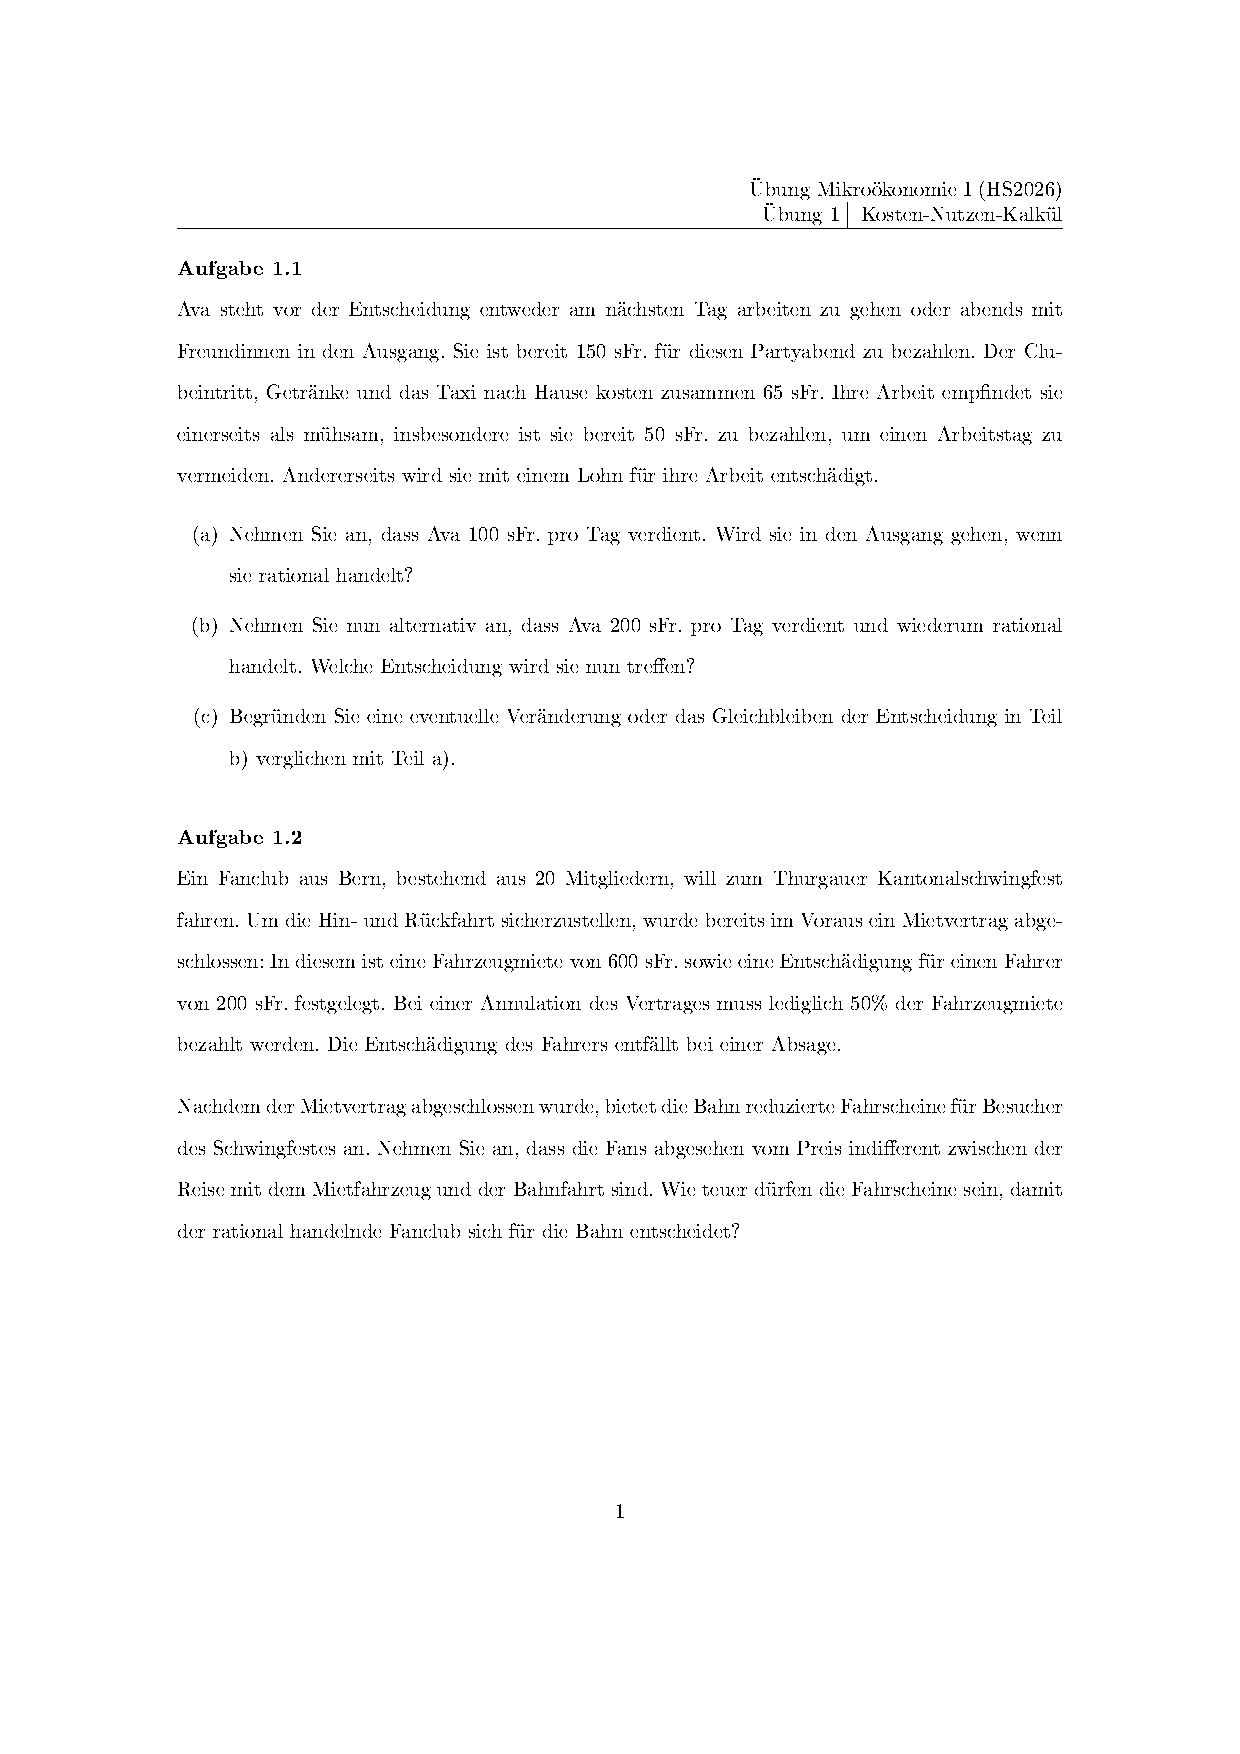
\includepdf[pages=-]{sheet.pdf}
   \exercise{1.1 Ausgang} \break
   \begin{itemize}
        \item Party = P 
        \item Arbeiten = A
        \item $ B(P) = 150$
        \item $ C(P) = 65$
   \end{itemize}
        
   \subexercise{a}
        \begin{itemize}
            \item $B(A) = 100$
            \item $C(A) = 50$
        \end{itemize}
        $B(P) - C(P) \ge B(P) - C(A)$
    \subexercise{b}
        \begin{itemize}
            \item $B(A) = 200$
            \item $C(A) = 50$
        \end{itemize}
        $B(P) - C(P) \le B(A) - C(A)$
    \subexercise{c}
        Die Nettonutzen von Arbeiten sind gestiegen, oder die Opportunitätskosten der Party sind gestiegen. Die Nettonutzen der Party sind relativ gesunken.
    \exercise{1.2}
        Gleich aber versunkenen Kosten des Buses (600/2 = 300) für alle Optionen oder keine der Optionen miteinbeziehen.
    \exercise{1.3 Technofestival}
    \subexercise{a}
    [x] = Tage
    [B(x)] = Franken
    [C(x)] = Franken
    \textbf{Nutzenfunktion}
    \begin{equation}
        B(x) = 100 + 100 * 0.75^x
    \end{equation}

    \textbf{Kostenfunktion}
    \begin{equation}
        C(x) = 65x
    \end{equation}

    \textbf{Nettonutzen Optimum}
    \begin{equation}
        N(x)_{max} = B(x) - C(x) \implies N'(x) = B'(x) - C'(x)= 0
    \end{equation}
    sodass 
    \begin{equation}
        N'(x) = -20 - (65) 
    \end{equation}
    \textbf{Richtige überlegung aber eigentlich ziemlich komplizierte Funktion einfacher ist:}
    \begin{enumerate}
        \item Tabelle machen
        \begin{itemize}
            \item Marginalbenefit (Nutzen für weitere Einheit oder die Ableitung bei der Einheit)
            \item Marginalcosts (MC)
            \item Benefits
            \item Costs
            \item Nettonutzen B-c
        \end{itemize}
        \item Ausfüllen
        \item Manuell auswerten wo $\textbf{B - C}$ am grössten ist.
    \end{enumerate}
    \subexercise{b}
     Für jede Tageinheit im Interval $[0,4]$ ist $MB > MC$ oder die ABleitung von B ist immer grösser 
    
\end{document}
 